\section*{Zielsetzung}
\label{sec:Zielsetzung}
In diesem Versuch soll der Übergang zwischen den Phasen flüssig und gasförmig quantitativ
untersucht werden. Ziel ist es, dabei die Dampfdruckkurve von Wasser im Bereich von
$\SI{30}{\milli\bar}$ bis $\SI{15}{\bar}$ zu bestimmen.

\section{Theorie}
\label{sec:Theorie}
Der anfangs verwendete Begriff der ``Phase`` beschreibt hierbei einen räumlich
abgegrenzten Bereich, in dem sich ein Stoff in einem physikalisch homogenen Zustand
befindet. Anschauliche Beispiele sind die Aggregatszustände.
\\
Die Unterteilung dieser Phasen kann im Zustandsdiagramm stattfinden, wo der Druck $p$
gegen die Temperatur $T$ aufgetragen wird. Für Wasser lassen sich dann mit drei Kurven
die drei Aggregatszustände abgrenzen:
\begin{figure}[H]
	\centering
	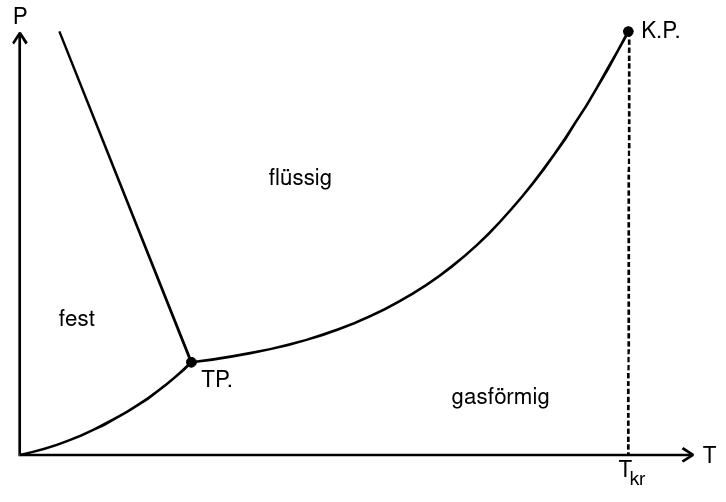
\includegraphics[height=8cm]{images/Zustandsdiagramm.png}
	\caption{Zustandsdiagramm des Wassers (nur qualitativ) \cite{anleitung}}
	\label{fig:zustandsdiagramm}
\end{figure}
\noindent
Offensichtlich kann innerhalb eines Aggregatszustandes $p$ und $T$ frei gewählt werden
(solange die Kombination noch im entsprechenden Zustand liegt), das System hat also zwei Freiheitsgrade.
Sind Druck und Temperatur jedoch so, dass der Zustand nahe an einer der Kurven ist, ändert
sich das. Dort existieren zwei Phasen nebeneinander. Für die sog. \textbf{Dampfdruckkurve}, die
zwischen Tripelpunkt und kritischem Punkt verläuft und die Aggregatszustände flüssig und
gasförmig trennt, hat das System dann auch nur noch einen Freiheitsgrad.
\\
Der Verlauf folgt hauptsächlich aus der \textbf{Verdampfungswärme $L$}, welche eine
charakteristische Eigenschaft für einen Stoff ist. Problematisch ist, dass $L$ nicht
konstant ist, sondern selbst auch temperaturabhängig ist. Es existiert jedoch ein
beschränkter Bereich, wo $L$ nahezu konstant ist. Dieser Bereich ist in diesem Versuch
von Interesse; dort soll die Dampfdruckkurve aufgenommen und $L$ bestimmt werden.

\subsection{Die mikroskopischen Vorgänge bei der Verdampfung und Kondensation}
\label{sec:Die mikroskopischen Vorgänge bei der Verdampfung und Kondensation}
Wird ein Gefäß mit Flüssigkeit evakuiert, so wird kurz nach der Evakuierung der Druck
wieder ansteigen. Das lässt sich dadurch erklären, dass ein Teil der Flüssigkeit in die
gasförmige Phase übergegangen ist. Dafür muss eine Arbeit gegen die Molekularkräfte aufgebracht
werden, welche aus dem Wärmevorrat der Flüssigkeit entnommen wird. Die für die Umwandlung
von einem Mol Flüssigkeit in Dampf gleicher Temperatur wird als molare Verdampfungswärme
$L$ bezeichnet. Die gasförmig frei beweglichen Moleküle können aber auch wieder auf die
Flüssigkeit treffen und dann teilweise kondensieren. Dabei geben sie ihre
Verdampfungswärme auch wieder ab. Beide Prozesse sind zufallsverteilt; nach längerer Zeit
kann sich jedoch ein Gleichgewicht einstellen, wo dann die Verdampfungsrate genau so hoch
ist wie die Kondensationsrate. Im Gleichgewichtszustand ist der Druck konstant, welcher
dann als \textbf{Sättigungsdampfdruck} bezeichnet wird. Da bei höheren Temperaturen die
Geschwindigkeitskurve der Moleküle in der Flüssigkeit auch ins schnellere verschoben wird,
benötigen diese nicht mehr so viel Energie um auszutreten. Daher steigt der
Sättigungsdruck mit der Temperatur an. 
\\
Der Sättigungsdampfdruck ist allerdings nicht volumenabhängig. Wird das Gasvolumen
vergrößert, so verdunstet auch mehr Flüssigkeit und es wird der gleiche Druck im
Gleichgewichtszustand erreicht.

\subsection{Ableitung einer Differentialgleichung für die Dampfdruckkurve}
\label{sec:Ableitung einer Differentialgleichung für die Dampfdruckkurve}


